\documentclass{article} % For LaTeX2e
\usepackage{forest}
\usepackage{url}
\usepackage{amsmath}
\usepackage{amsfonts}
% \usepackage{algorithm}
\usepackage{algorithm2e}
\usepackage{graphicx}
\usepackage{color}
\usepackage{listings}
\usepackage{verbatim}
\usepackage[letterpaper, margin=0.95in]{geometry}

\usepackage[parfill]{parskip}
% \usepackage{minted}
\usepackage{enumitem}

\newcommand{\bs}{\mathbf{s}}
\newcommand{\ba}{\mathbf{a}}
\newcommand{\bA}{\mathbf{A}}

\newtheorem{definition}{Definition}[section]
\newtheorem{proposition}{Proposition}[section]
\newtheorem{lemma}{Lemma}[section]
\newtheorem{assumption}{Assumption}[section]
\newtheorem{theorem}{Theorem}[section]
\newtheorem{corollary}{Corollary}[section]

\newcommand{\checkeditem}[2]{\edef\x{0#1}\item[\expandafter\filled\x|#2]}

\usepackage{hyperref}
\hypersetup{
    colorlinks=true,
    linkcolor=blue,
    filecolor=magenta,      
    urlcolor=blue,
}

\usepackage{courier}
 
\definecolor{codegreen}{rgb}{0,0.6,0}
\definecolor{codegray}{rgb}{0.5,0.5,0.5}
\definecolor{codepurple}{rgb}{0.58,0,0.82}
\definecolor{backcolour}{rgb}{0.95,0.95,0.92}

\lstdefinestyle{mystyle}{
    backgroundcolor=\color{backcolour},   
    commentstyle=\color{codegreen},
    keywordstyle=\color{magenta},
    numberstyle=\tiny\color{codegray},
    stringstyle=\color{codepurple},
    basicstyle=\footnotesize\ttfamily,
    breakatwhitespace=false,         
    breaklines=true,                 
    captionpos=b,                    
    keepspaces=true,                 
    %numbers=left,                    
    numbersep=5pt,                  
    showspaces=false,                
    showstringspaces=false,
    showtabs=false,                  
    tabsize=2
}

\lstset{style=mystyle}

\newcommand{\cmt}[1]{{\footnotesize\textcolor{red}{#1}}}
\newcommand{\todo}[1]{\cmt{TO-DO: #1}}

%% One of the nicest things about LaTeX is you can create custom macros. If  there is a long-ish expression that you will write often, it is nice to give it a shorter command.
%% For our common number systems.
\newcommand{\R}{\mathbb{R}} %% The blackboard-bold R that you have seen used for real numbers is typeset by $\mathbb{R}$. This macro means that $\RR$ will yield the same result, and is much shorter to type.
\newcommand{\N}{\mathbb{N}}
\newcommand{\Z}{\mathbb{Z}} 
\newcommand{\Q}{\mathbb{Q}}
\newcommand{\E}{\mathbb{E}}
\newcommand{\C}{\mathbb{C}}
\newcommand{\Lbb}{\mathbb{L}}
\newcommand{\Prob}{\mathbb{P}}
\newcommand{\Afancy}{\mathcal{A}}
\newcommand{\Bfancy}{\mathcal{B}}
\newcommand{\Cfancy}{\mathcal{C}}
\newcommand{\Dfancy}{\mathcal{D}}
\newcommand{\Efancy}{\mathcal{E}}
\newcommand{\Ffancy}{\mathcal{F}}
\newcommand{\Gfancy}{\mathcal{G}}
\newcommand{\Hfancy}{\mathcal{H}}
\newcommand{\Ifancy}{\mathcal{I}}
\newcommand{\Jfancy}{\mathcal{J}}
\newcommand{\Kfancy}{\mathcal{K}}
\newcommand{\Lfancy}{\mathcal{L}}
\newcommand{\Mfancy}{\mathcal{M}}
\newcommand{\Nfancy}{\mathcal{N}}
\newcommand{\Ofancy}{\mathcal{O}}
\newcommand{\Pfancy}{\mathcal{P}}
\newcommand{\Qfancy}{\mathcal{Q}}
\newcommand{\Rfancy}{\mathcal{R}}
\newcommand{\Sfancy}{\mathcal{S}}
\newcommand{\Tfancy}{\mathcal{T}}
\newcommand{\Ufancy}{\mathcal{U}}
\newcommand{\Vfancy}{\mathcal{V}}
\newcommand{\Wfancy}{\mathcal{W}}
\newcommand{\Xfancy}{\mathcal{X}}
\newcommand{\Yfancy}{\mathcal{Y}}
\newcommand{\Zfancy}{\mathcal{Z}}
\renewcommand{\thempfootnote}{\arabic{mpfootnote}}

\newcommand{\var}{\text{var}}
\newcommand{\cov}{\text{cov}}

\newcommand{\argmin}{\text{arg}\,\text{min}}
\newcommand{\indep}{\perp \!\!\! \perp}


\newcommand\abs[1]{\left| #1 \right|} %% This will do the same but with vertical bars. I.e., \abs{STUFF} gives |STUFF|
\newcommand\parens[1]{\left( #1 \right)} %% Similar. \parens{STUFF} gives (STUFF)
\newcommand\brac[1]{\left[ #1 \right]} %% Similar. \brac{STUFF} gives [STUFF]
\newcommand\solution[1]{\begin{mdframed}
\emph{Solution.} #1
\end{mdframed}}
\newcommand\solutionproof[1]{\begin{mdframed}
\begin{proof} #1
\end{proof}
\end{mdframed}}

\newcommand{\red}{\color{red}}
\definecolor{darkblue}{rgb}{0.2, 0.2, 0.5}
\newcommand{\sol}{~\color{darkblue}{\bf Solution:~}}

\title{CS285 Deep Reinforcement Learning HW4: Model-Based RL\\
\textbf{Due November 3rd, 11:59 pm}}

\author{}
\date{}

\begin{document}

\maketitle

%%%%%%%%%%%%%%%%%%%%%%%%%%%%%%%%%%%%%%%%%%%%%%%%%%%%%%%%%%%%%

\section{Introduction}

The goal of this assignment is to get experience with model-based reinforcement learning. In general, model-based RL consists of two main parts: learning a dynamics function to model observed state transitions, and then using predictions from that model in some way to decide what to do (e.g., use model predictions to learn a policy, or use model predictions directly in an optimization setup to maximize predicted rewards).

In this assignment, you will get both theoretical and practical experience with model-based RL. In the analysis section, you will analyze the effectiveness of a simple count-based model. Before doing that section, it will be greatly beneficial to first go over lecture 17 of this course on basics of RL theory (if you wish to complete this section before the lecture, the same lecture from past years will be sufficient); another beneficial resource will be section 2 of this \href{https://rltheorybook.github.io/rltheorybook_AJKS.pdf}{textbook}.  
Then, in the coding section, you will implement both the process of learning a dynamics model, as well as the process of creating a controller to perform action selection through the use of these model predictions. For references to this type of approach, see this \href{https://arxiv.org/pdf/1708.02596.pdf}{paper} and this \href{https://arxiv.org/pdf/1909.11652.pdf}{paper}.

%%%%%%%%%%%%%%%%%%%%%%%%%%%%%%%%%%%%%%%%%%%%%%%%%%%%%%%%%%%%%

\newpage

\section{Analysis}

\paragraph{Setting.} We have a discounted tabular MDP $M =(\mathcal{S}, \mathcal{A}, P, r, \gamma)$ where $\mathcal{S}$, $\mathcal{A}$ are a finite set of states and actions, $P$ is the dynamics model (where $P(\cdot \mid s, a)$ is a probability distribution over states), $r$ is a reward function (where rewards are between $[0, 1]$), and $\gamma \in (0, 1)$ is the discount factor. 


\paragraph{Learning a dynamics model.} We consider the most naive model-based algorithm. Suppose we have access to a simulator of the environment, and at each state-action pair $(s, a)$, we call our simulator $N$ times retrieving samples $s' \sim P(\cdot \mid s, a)$. Then, we build a dynamics model of the environment as simply:
$$
\widehat{P}(s' \mid s, a) = \frac{\mathsf{count}(s, a, s')}{N}
$$
where $\mathsf{count}(s, a, s')$ is the number of times we observed $(s, a)$ transitioning to $s'$. 
For tabular MDP $M$, we can view $\widehat{P}$ as a matrix of size $|\mathcal{S}||\mathcal{A}| \times |\mathcal{S}|$. 

\paragraph{Additional notation.} Let $\widehat{M}$ be an MDP identical to $M$, except where the true dynamics $P$ is replaced by model $\widehat{P}$. Let $\widehat{V}^\pi$, $\widehat{Q}^\pi$, $\widehat{V}^*$, and $\widehat{Q}^*$ denote the value function and state-action value function, and optimal value and state-action value function, in $\widehat{M}$, respectively. 


\paragraph{Problem 2.1.} 
In lecture 17, we saw a proof of a lemma called the \emph{Simulation Lemma}, which states that for any policy $\pi$:
\begin{align*}
Q^\pi - \widehat{Q}^\pi = \gamma(I - \gamma \widehat{P}^\pi)^{-1} (P - \widehat{P}) V^\pi\,.
\end{align*}
Prove the following similar lemma, which we dub the \emph{Alternative Simulation Lemma}:

\emph{
(Alternative Simulation Lemma) For any policy $\pi$, we have:}
\begin{align*}
   Q^\pi - \widehat{Q}^\pi = \gamma(I - \gamma P^\pi)^{-1} (P - \widehat{P}) \widehat{V}^\pi\,. 
\end{align*}

\begin{sol}
    We prove the Alternative Simulation Lemma as follows:
    \begin{align*}
        Q^\pi - \hat{Q}^\pi &= (I - \gamma P^\pi)^{-1} r - \hat{Q}^\pi \\
        &= (I - \gamma P^\pi)^{-1} \left(r - (I - \gamma P^\pi) \hat{Q}^\pi\right) \\
        &= (I - \gamma P^\pi)^{-1} \left((I - \gamma \hat{P}^\pi)\hat{Q}^\pi - (I - \gamma P^\pi) \hat{Q}^\pi\right) \\
        &= (I - \gamma P^\pi)^{-1} \left( \gamma(P^\pi - \hat{P}^\pi) \hat{Q}^\pi\right) \\
        &= \gamma(I - \gamma P^\pi)^{-1} (P - \hat{P}) \Pi \hat{Q}^\pi \\
        &= \gamma(I - \gamma P^\pi)^{-1} (P - \hat{P}) \hat{V}^\pi
    \end{align*}
\end{sol}


\newpage\paragraph{Problem 2.2} 
In lecture 17, we saw how to bound $||Q^\pi - \widehat{Q}^\pi||_{\infty}$ using the Simulation Lemma and standard concentration arguments. We will attempt to do the same with the Alternative Simulation Lemma derived in Problem 2.1. Which of the following statements (may be multiple) are correct?

\emph{Hint: A statement is correct if the inequalities referenced are applied correctly, and if their assumptions hold before applying them.}

\emph{Hint 2: For each observed transition from $(s, a)$ to $s'$, you can define a random variable $X = \mathbb{I}_{s'} \cdot V$ that is the dot product between $\mathbb{I}_{s'} \in \mathbb{R}^{|\mathcal{S}|}$ an indicator vector at $s'$ and vector $V \in \mathbb{R}^{|\mathcal{S}|}$, and whose expected value is $\mathbb{E}[X] = P(\cdot \mid s, a) \cdot V$. What does Hoeffding's inequality look like when applied to all $N$ observed transitions from $(s, a)$ in this way? Can Hoeffding's inequality be applied for any vector $V$?}
\begin{itemize}[leftmargin=0.2in]
    \item[1.] For any policy $\pi$ and $\delta > 0$, the following holds with probability at least $1 - \delta$,
    \begin{align*}
    ||(P - \widehat{P}) \widehat{V}^\pi||_{\infty}
    &\leq 
    \max_{s, a} ||P(\cdot \mid s, a) - \widehat{P}(\cdot \mid s, a)||_{1} ||\widehat{V}^\pi||_{\infty} \\
    &\leq 
    \frac{1}{1 - \gamma} \sqrt{\frac{4|S| \log (|\mathcal{S}||\mathcal{A}|/\delta)}{N}}\,,
    \end{align*}
    where we use Hoeffding's inequality and the union bound in the second inequality.
    
    \begin{sol}
        This statement is \textbf{correct}. Note that from lecture, we have that 
        \[\|P(\cdot \mid s, a) - \hat{P}(\cdot \mid s, a)\|_1 \leq c \sqrt{\frac{|\mathcal{S}| \log (1/\delta)}{N}}\]
        for some constant $c$ with probability $1 - \delta$. Then, let us use $c = 2$ and apply a union bound to obtain the following: 
        \[P\left(\max_{s, a} \|P(\cdot \mid s, a) - \hat{P}(\cdot \mid s, a)\|_1 > 2 \sqrt{\frac{|S| \log (1/\delta^*)}{N}}\right) \leq |\mathcal{S}||\mathcal{A}| \delta^*.\]
        We want the RHS to be a single term $\delta$, so we substitute $\delta^* = \frac{\delta}{|S||A|}$ to get 
        \[P\left(\max_{s, a} \|P(\cdot \mid s, a) - \hat{P}(\cdot \mid s, a)\|_1 > 2 \sqrt{\frac{|S| \log (|\mathcal{S}||\mathcal{A}| / \delta)}{N}}\right) \leq |\mathcal{S}||\mathcal{A}| \cdot \frac{\delta}{|\mathcal{S}||\mathcal{A}|} = \delta,\]
        and taking the complement gives 
        \[P\left(\max_{s, a} \|P(\cdot \mid s, a) - \hat{P}(\cdot \mid s, a)\|_1 \leq \sqrt{\frac{4|S| \log (|\mathcal{S}||\mathcal{A}| / \delta)}{N}}\right) \geq 1 - \delta.\]
        \[P\left(\max_{s, a} \|P(\cdot \mid s, a) - \hat{P}(\cdot \mid s, a)\|_1 \|\hat{V}^\pi\|_\infty \leq \sqrt{\frac{4|\mathcal{S}| \log (|\mathcal{S}||\mathcal{A}| / \delta)}{N}} \|\hat{V}^\pi\|_\infty\right) \geq 1 - \delta.\]
        Thus, we conclude that 
        \begin{align*}
            ||(P - \widehat{P}) \widehat{V}^\pi||_{\infty}
            &\leq 
            \max_{s, a} ||P(\cdot \mid s, a) - \widehat{P}(\cdot \mid s, a)||_{1} ||\widehat{V}^\pi||_{\infty} \\
            &\leq \sqrt{\frac{4|\mathcal{S}| \frac{|\Sfancy||\Afancy|}{\delta}}{N}} \|\hat{V}^\pi\|_\infty \\
            &\leq 
            \frac{1}{1 - \gamma} \sqrt{\frac{4|S| \log (|\mathcal{S}||\mathcal{A}|/\delta)}{N}}\,,
            \end{align*}
        with probability at least $1 - \delta$. 
    \end{sol}

    \newpage

    \item[2.] For any policy $\pi$ and $\delta > 0$, the following holds with probability at least $1 - \delta$,
    \begin{align*}
    ||(P - \widehat{P}) \widehat{V}^\pi||_{\infty}
    &\leq 
    \frac{1}{1 - \gamma} \sqrt{\frac{2|\mathcal{S}| \log(2|\mathcal{S}||\mathcal{A}|/\delta)}{N}}\,,
    \end{align*}
    using Hoeffding's inequality and the union bound.

    \begin{sol}
        This statement is \textbf{incorrect}. Since $\hat{V}^\pi$ depends on the observed transitions, we cannot use Hoeffding's inequality. 
    \end{sol}

    \item[3.] For $\delta > 0$, the following holds with probability at least $1 - \delta$,
    \begin{align*}
    ||(P - \widehat{P}) V^*||_{\infty} 
    \leq 
    \frac{1}{1- \gamma} \sqrt{\frac{2 \log(2|\mathcal{S}||\mathcal{A}|/\delta)}{N}}\,,
    \end{align*}
    where the inequality arises from Hoeffding's inequality and the union bound.

    \begin{sol}
        This statement is \textbf{correct}. Since $V^*$ is independent of the observed transitions, we can apply Hoeffding's inequality to derive this result; the procedure is similar to that in (1).
    \end{sol}

    \item[4.] For $\delta > 0$, the following holds with probability at least $1 - \delta$,
    \begin{align*}
    ||(P - \widehat{P}) \widehat{V}^*||_{\infty} 
    \leq 
    \frac{1}{1- \gamma} \sqrt{\frac{2 \log(2|\mathcal{S}||\mathcal{A}|/\delta)}{N}}\,,
    \end{align*}
    where we use Hoeffding's inequality and the union bound.

    \begin{sol}
        This statement is \textbf{incorrect}. Since $\hat{V}^*$ depends on the observed transitions, we cannot use Hoeffding's inequality. 
    \end{sol}
\end{itemize}

\newpage

%%%%%%%%%%%%%%%%%%%%%%%%%%%%%%%%%%%%%%%%%%%%%%%%%%%%%%%%%%%%%
\section{Model-Based Reinforcement Learning}

We will now provide a brief overview of model-based reinforcement learning (MBRL), and the specific type of MBRL you will be implementing in this homework. Please see \href{http://rail.eecs.berkeley.edu/deeprlcourse/static/slides/lec-11.pdf}{Lecture 11: Model-Based Reinforcement Learning} (with specific emphasis on the slides near page 9) for additional details.

MBRL consists primarily of two aspects: (1) learning a dynamics model and (2) using the learned dynamics models to plan and execute actions that minimize a cost function (or maximize a reward function).

\subsection{Dynamics Model}

In this assignment, you will learn a neural network dynamics model $f_\theta$ of the form
\begin{align}
\hat{\Delta}_{t+1} &= f_\theta(\bs_t, \ba_t)
\end{align}
which predicts the change in state given the current state and action. So given the prediction $\hat{\Delta}_{t+1}$, you can generate the next prediction with
\begin{align}
\hat{\bs}_{t+1} &= \bs_t + \hat{\Delta}_{t+1} .
\end{align}
% In other words, the neural network $f_\theta$ encodes the change in state that occurs as a result of executing the action $\ba_t$ from state $\bs_t$. 
See the previously \href{https://arxiv.org/pdf/1708.02596.pdf}{referenced paper} for intuition on why we might want our network to predict state differences, instead of directly predicting next state.

You will train $f_\theta$ in a standard supervised learning setup, by performing gradient descent on the following objective:
\begin{align}
\mathcal{L}(\theta) &= \sum_{(\bs_t, \ba_t, \bs_{t+1}) \in \mathcal{D}} \| (\bs_{t+1} - \bs_t) - f_\theta(\bs_t, \ba_t) \|_2^2 \\
&= \sum_{(\bs_t, \ba_t, \bs_{t+1}) \in \mathcal{D}} \| \Delta_{t+1} - \hat{\Delta}_{t+1} \|_2^2 \label{eqn:train-dynamics}
\end{align}

In practice, it's helpful to normalize the target of a neural network.
So in the code, we'll train the network to predict a \emph{normalized} version of the change in state, as in
\begin{align}
\mathcal{L}(\theta) &= \sum_{(\bs_t, \ba_t, \bs_{t+1}) \in \mathcal{D}} \| \text{Normalize}(\bs_{t+1} - \bs_t) - f_\theta(\bs_t, \ba_t) \|_2^2.
\end{align}
Since $f_\theta$ is trained to predict the normalized state difference, you generate the next prediction with
\begin{align}
\hat{\bs}_{t+1} &= \bs_t + \text{Unnormalize}(f_\theta(\bs_t, \ba_t)).
\end{align}

\subsection{Action Selection}

Given the learned dynamics model, we now want to select and execute actions that minimize a known cost function (or maximize a known reward function). Ideally, you would calculate these actions by solving the following optimization:
\begin{align}
\ba_t^* &= \arg\min_{\ba_{t:\infty}} \sum_{t'=t}^\infty c(\hat{\bs}_{t'}, \ba_{t'}) \;\;\text{where}\;\; \hat{\bs}_{t'+1} = \hat{\bs}_{t'} + f_\theta(\hat{\bs}_{t'}, \ba_{t'}). \label{eqn:action-selection-full}
\end{align}
However, solving Eqn.~\ref{eqn:action-selection-full} is impractical for two reasons: (1) planning over an infinite sequence of actions is impossible and (2) the learned dynamics model is imperfect, so using it to plan in such an open-loop manner will lead to accumulating errors over time and planning far into the future will become very inaccurate. 

Instead, one alternative is to solve the following gradient-free optimization problem:
\begin{align}
\bA^* &= \arg\min_{\{\bA^{(0)}, ..., \bA^{(K-1)}\}} \sum_{t'=t}^{t+H-1} c(\hat{\bs}_{t'}, \ba_{t'}) \;\;\text{s.t.}\;\; \hat{\bs}_{t'+1} = \hat{\bs}_{t'} + f_\theta(\hat{\bs}_{t'}, \ba_{t'}), \label{eqn:action-selection-mpc}
\end{align}
in which $\bA^{(k)} = (a_t^{(k)}, \dots, a_{t+H-1}^{(k)})$ are each a random action sequence of length $H$. What Eqn.~\ref{eqn:action-selection-mpc} says is to consider $K$ random action sequences of length $H$, predict the result (i.e., future states) of taking each of these action sequences using the learned dynamics model $f_\theta$, evaluate the cost/reward associated with each candidate action sequence, and select the best action sequence. Note that this approach only plans $H$ steps into the future, which is desirable because it prevent accumulating model error, but is also limited because it may not be sufficient for solving long-horizon tasks. 

A better alternative to this random-shooting optimization approach is the cross-entropy method (CEM), which is similar to random-shooting, but with iterative improvement of the distribution of actions that are sampled from. We first randomly initialize a set of $K$ action sequences $\bA^{(0)}, ..., A^{(K-1)}$, like in random-shooting. Then, we choose the $J$ sequences with the highest predicted sum of discounted rewards as the "elite" action sequences. We then fit a diagonal Gaussian with the same mean and variance as the "elite" action sequences, and use this as our action sampling distribution for the next iteration. After repeating this process $M$ times, we take the final mean of the Gaussian as the optimized action sequence. See Section 3.3 in this \href{https://arxiv.org/pdf/1909.11652.pdf}{paper} for more details.

Additionally, since our model is imperfect and things will never go perfectly according to plan, we adopt a model predictive control (MPC) approach, where at every time step we perform random-shooting or CEM to select the best $H$-step action sequence, but then we execute only the first action from that sequence before replanning again at the next time step using updated state information. This reduces the effect of compounding errors when using our approximate dynamics model to plan too far into the future.


\subsection{On-Policy Data Collection}

Although MBRL is in theory off-policy---meaning it can learn from any data---in practice it will perform poorly if you don't have on-policy data. In other words, if a model is trained on only randomly-collected data, it will (in most cases) be insufficient to describe the parts of the state space that we may actually care about. We can therefore use on-policy data collection in an iterative algorithm to improve overall task performance. This is summarized as follows:

\begin{algorithm}[H]
 \caption{Model-Based RL with On-Policy Data}
\SetAlgoLined
  Run base policy $\pi_0(\ba_t, \bs_t)$ (e.g., random policy) to collect $\mathcal{D} = \{(\bs_t, \ba_t, \bs_{t+1})\}$ \\
  \While{not done}{
    Train $f_\theta$ using $\mathcal{D}$ (Eqn.~\ref{eqn:train-dynamics}) \\
    $\bs_t \leftarrow$ current agent state \\
    \For{\text{rollout number} $m=0$ to $M$}{
        \For{\text{timestep} $t=0$ to $T$}{
          $\bA^* = \pi_{\text{MPC}}(\ba_t, \bs_t)$ where $\pi_{\text{MPC}}$ is obtained from random-shooting or CEM\\
          $\ba_t \leftarrow$ first action in $\bA^*$ \\
          Execute $\ba_t$ and proceed to next state $\bs_{t+1}$ \\
          Add $(\bs_t, \ba_t, \bs_{t+1})$ to $\mathcal{D}$
        }
    }
  }
\end{algorithm}

\subsection{Ensembles}
A simple and effective way to improve predictions is to use an ensemble of models.
The idea is simple: rather than training one network $f_\theta$ to make predictions, we'll train $N$ independently initialized networks $\{f_{\theta_n}\}_{n=1}^N$. At test time, for each candidate action sequence, we'll generate $N$ independent rollouts and average the rewards of these rollouts to choose the best action sequence.



%%%%%%%%%%%%%%%%%%%%%%%%%%%%%%%%%%%%%%%%%%%%%%%%%%%%%%%%%%%%%
\newpage
\section{Code}

You will implement the MBRL algorithm described in the previous section.

\subsection{Overview}

Obtain the code from \url{https://github.com/berkeleydeeprlcourse/homework_fall2023/tree/master/hw4}. You will be implementing a model-based RL agent in \texttt{cs285/agents/model\_based\_agent.py}. Make sure to also read the following files:
\begin{itemize}
    \item \texttt{cs285/env\_configs/mpc\_config.py}: generates all of the configuration for the model-based agent.
\end{itemize}

%%%%%%%%%%%%%%%%%%%%%%%%%%%%%%%%%%%%%%%%%%%%%%%%%
%%%%%%%%%%%%%%%%%%%%%%%%%%%%%%%%%%%%%%%%%%%%%%%%%

\newpage
\section*{Problem 1}

\underline{What you will implement:}\\
Collect a large dataset by executing random actions. Train a neural network dynamics model on this fixed dataset. The implementation that you will do here will be for training the dynamics model.

\underline{What code files to fill in:}
\begin{enumerate}
    \item \verb+cs285/agents/model_based_agent.py+: up to (and including) \verb+update_statistics+.
    \item \verb+cs285/scripts/run_hw4.py+: everything except for \verb+collect_mbpo_rollout+ at the top of the file.
\end{enumerate}


\underline{What command to run:}
\begin{lstlisting}[escapechar=@]
python cs285/scripts/run_hw4.py -cfg experiments/mpc/halfcheetah_0_iter.yaml
\end{lstlisting}

This config will only run the first iteration without actually evaluating the policy, meaning it will only train the ensemble of dynamics models. The code will produce plots inside your logdir that illustrate the full learning curve of the dynamics models. For the first command, the loss should go below 0.2 by iteration 500. 

Modify \verb+experiments/mpc/halfcheetah_0_iter.yaml+ to change some hyperparameters. Try at least two other configurations of hyperparameters that affect dynamics model training (e.g., number of layers, hidden size, or learning rate).

\underline{What to submit:} For this question, submit the learning curve for 3 runs total: the initial run with provided hyperparameters as well as 2 of your own. 
% (a) these runs as part of your run\_logs, \\
% (b) qualitative model prediction plots for the 2 network sizes (runs 1,2) \\
% (c) qualitative model prediction plots for the number of training steps (runs 2,3)
% (d) explicitly report the final loss value (approximate, from losses.png) as well as H-step MPE value (from title of predictions.png) for each of the runs above. Rank these runs in order of worst to best H-step model predictions. State your intuition about why/what's happening for each of the two trends we are examining. Why does it make sense for training loss to improve but for the H-step model predictions to worsen? Assuming we do NOT want to change our model itself (e.g., to predict more steps into the future), what should we be taking into consideration when training these models, aside from training loss alone? \\

Note that for these learning curves, we intend for you to just copy the png images produced by the code.

\begin{sol}
  Here are the learning curves for the initial run with provided hyperparameters, with number of layers modified to 10, and with learning rate modified to 0.01 (respectively):
  \begin{figure}[!ht]
    \begin{center}
    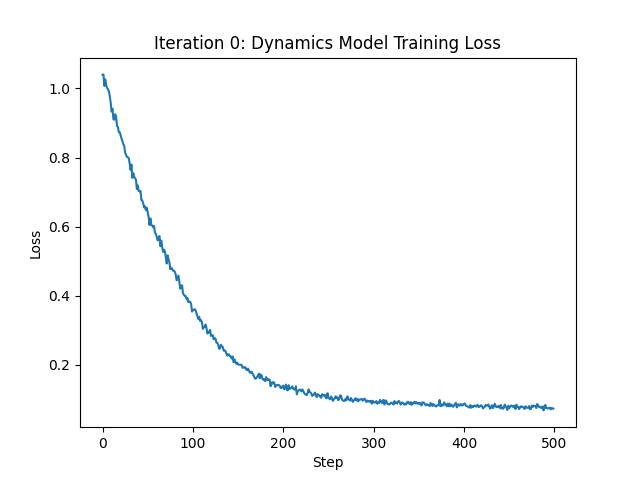
\includegraphics[width=2.1in]{images/q1/itr_0_loss_curve.png}
    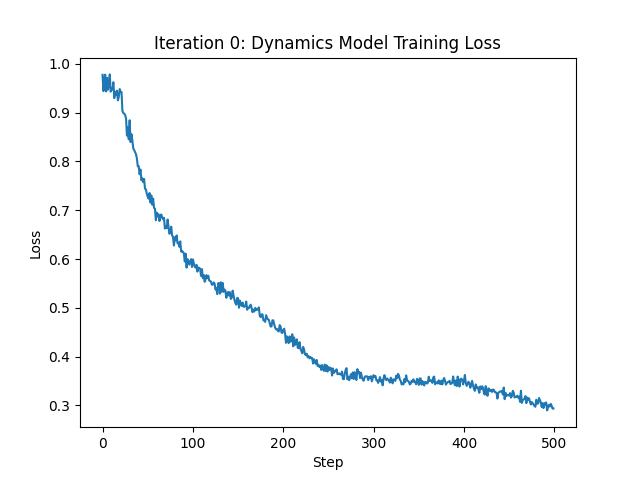
\includegraphics[width=2.1in]{images/q1/itr_0_loss_curve_layer10.png}
    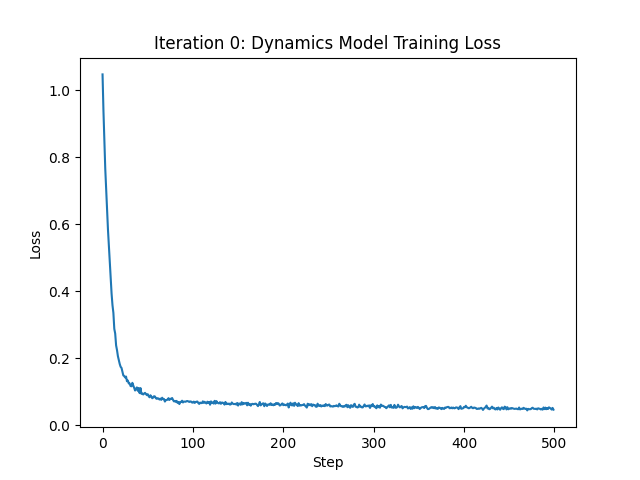
\includegraphics[width=2.1in]{images/q1/itr_0_loss_curve_lr0.01.png}
  \end{center}
  \caption{Based on the middle plot, it seems that increasing the number of layers to 10 is highly detrimental to convergence of the loss. On the other hand, looking at the right figure, we see that increasing the learning rate to 0.01 improves the speed of convergence for this task.}
  \end{figure}
\end{sol}
%%%%%%%%%%%%%%%%%%%%%%%%%%%%%%%%%%%%%%%%%%%%%%%%%
%%%%%%%%%%%%%%%%%%%%%%%%%%%%%%%%%%%%%%%%%%%%%%%%%

\newpage
\section*{Problem 2}

\underline{What will you implement:}\\ 
Action selection using your learned dynamics model and a given reward function.

\underline{What code files to fill in:}
\begin{enumerate}
    \item \verb+cs285/agents/model_based_agent.py+: the rest of the file, except for the CEM strategy in \verb+get_action+.
\end{enumerate}

\underline{What commands to run:}\\
\begin{lstlisting}[escapechar=@]
python cs285/scripts/run_hw4.py -cfg experiments/mpc/obstacles_1_iter.yaml
\end{lstlisting}

Recall the overall flow of our training loop. We first collect data with our policy (which starts as random), we train our model on that collected data, we evaluating the resulting MPC policy (which now uses the trained model), and repeat.
To verify that your MPC is indeed doing reasonable action selection, run one iteration of this process using the command above.
This will evaluate your MPC policy, but not use it to collect data for future iterations.
Look at \verb+eval_return+, which should be greater than -70 after one iteration.

\underline{What to submit:}\\
Submit this run as part of your run\_logs, and report your \verb+eval_return+.

\begin{sol}
  My MPC policy achieved an average eval return of -41.337.
\end{sol}
%%%%%%%%%%%%%%%%%%%%%%%%%%%%%%%%%%%%%%%%%%%%%%%%%
%%%%%%%%%%%%%%%%%%%%%%%%%%%%%%%%%%%%%%%%%%%%%%%%%

\newpage
\section*{Problem 3}

\underline{What will you implement:}\\ \\
MBRL algorithm with on-policy data collection and iterative model training.

\underline{What code files to fill in:}\\ \\
None. You should already have done everything that you need, because \verb+run_hw4.py+ already aggregates your collected data into a replay buffer. Thus, iterative training means to just train on our growing replay buffer while collecting new data at each iteration using the most newly trained model.

\underline{What commands to run:}
\begin{lstlisting}[escapechar=@]
python cs285/scripts/run_hw4.py -cfg experiments/mpc/obstacles_multi_iter.yaml

python cs285/scripts/run_hw4.py -cfg experiments/mpc/reacher_multi_iter.yaml

python cs285/scripts/run_hw4.py -cfg experiments/mpc/halfcheetah_multi_iter.yaml
\end{lstlisting}

You should expect rewards of around -25 to -20 for the obstacles env, rewards of around -300 to -250 for the reacher env, and rewards of around 250-350 for the cheetah env.

\underline{What to submit:}\\
Submit these runs as part of your run\_logs, and include the return plots in your pdf.

\begin{sol}
  We plot the eval return of MBRL on Obstacles below:
  \begin{center}
    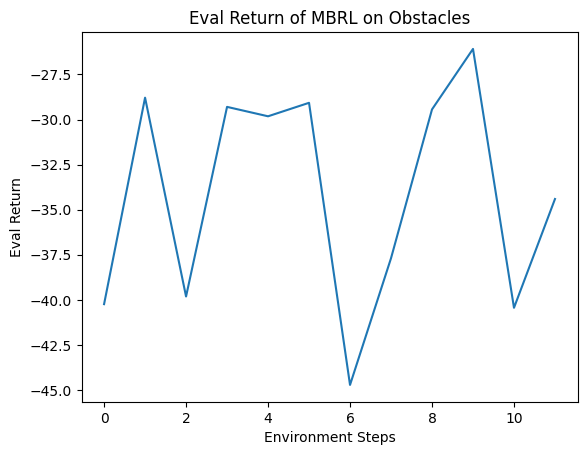
\includegraphics[width=4in]{images/q3/obstacles.png}
  \end{center}
  We plot the eval return of MBRL on Reacher below:
  \begin{center}
    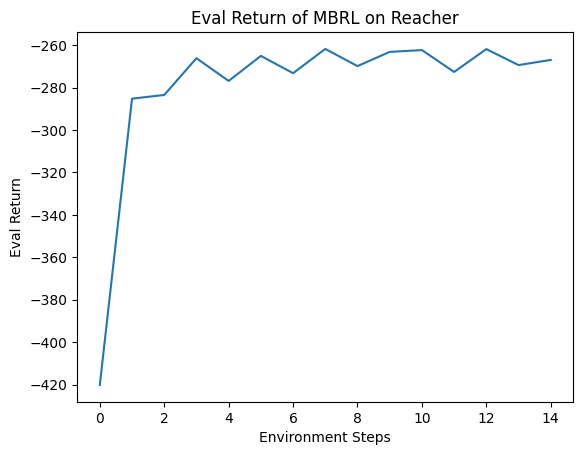
\includegraphics[width=4in]{images/q3/reacher.png}
  \end{center}
  We plot the eval return of MBRL on HalfCheetah below:
  \begin{center}
    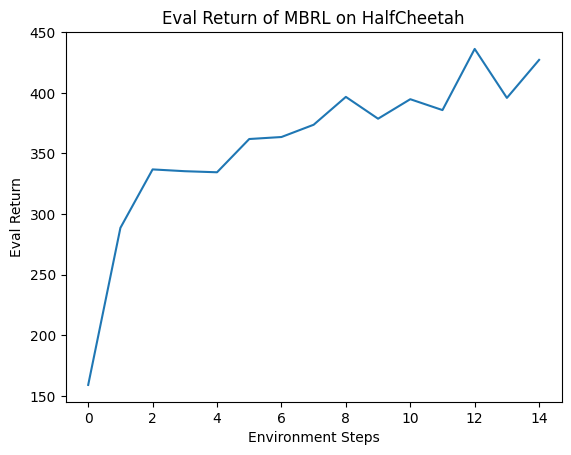
\includegraphics[width=4in]{images/q3/cheetah.png}
  \end{center}
\end{sol}
%%%%%%%%%%%%%%%%%%%%%%%%%%%%%%%%%%%%%%%%%%%%%%%%%
%%%%%%%%%%%%%%%%%%%%%%%%%%%%%%%%%%%%%%%%%%%%%%%%%

\newpage
\section*{Problem 4}

\underline{What will you implement:}\\ 
You will compare the performance of your MBRL algorithm as a function of three hyperparameters: the number of models in your ensemble, the number of random action sequences considered during each action selection, and the MPC planning horizon.

\underline{What code files to fill in:}\\
None.

\underline{What commands to run:}\\
\begin{lstlisting}[escapechar=@]
python cs285/scripts/run_hw4.py -cfg experiments/mpc/reacher_ablation.yaml
\end{lstlisting}

Modify (or make copies of) the YAML file to ablate each of the hyperparameters. For each hyperparameter, do at least 1 run with it increased and 1 with it decreased from the default (so 7 runs total). Make sure to keep the other hyperparameters the same when studying the effect of one of them.

\underline{What to submit:}
\begin{enumerate}
    \item Submit these runs as part of your run\_logs.
    \item Include the following plots (as well as captions that describe your observed trends) of the following:
\begin{itemize}
    \item effect of ensemble size
    \item effect of the number of candidate action sequences
    \item effect of planning horizon
\end{itemize}
\end{enumerate}

Be sure to include titles and legends on all of your plots. \\

%%%%%%%%%%%%%%%%%%%%%%%%%%%%%%%%%%%%%%%%%%%%%%%%%
%%%%%%%%%%%%%%%%%%%%%%%%%%%%%%%%%%%%%%%%%%%%%%%%%

\newpage
\section*{Problem 5}

\underline{What will you implement:}\\ 
You will compare the performance of your MBRL algorithm with action selecting performed by random-shooting (what you have done up to this point) and CEM.

Because CEM can be much slower than random-shooting, we will only run MBRL for 5 iterations for this problem. We will try two hyperparameter settings for CEM and compare their performance to random-shooting.

\underline{What code files to fill in:}
\begin{enumerate}
    \item \verb+cs285/agents/model_based_agent.py+: the CEM action selection strategy.
\end{enumerate}

\underline{What commands to run:}\\
\begin{lstlisting}[escapechar=@]
python cs285/scripts/run_hw4.py -cfg experiments/mpc/halfcheetah_cem.yaml
\end{lstlisting}

You should expect rewards around 800 or higher when using CEM on the cheetah env. Try a \verb+cem_num_iters+ value of both 2 and 4, and compare results.

\underline{What to submit:}\\
1) Submit these runs as part of your run\_logs.\\ \\
2) Include a plot comparing random shooting (from Problem 3) with CEM, as well as captions that describe how CEM affects results for different numbers of sampling iterations (2 vs. 4).

%%%%%%%%%%%%%%%%%%%%%%%%%%%%%%%%%%%%%%%%%%%%%%%%%%%%%%%%%%%%%

\newpage
\section*{Problem 6}

\underline{What will you implement:}\\ 

In this homework you will also be implementing a variant of \href{https://arxiv.org/pdf/1906.08253}{MBPO}. Another way of leveraging the learned model is through generating additional samples to train the policy and value functions. Since RL often requires many environment interaction samples, which can be costly, we can use our learned model to generate additional samples to improve sample complexity. In MBPO, we build on your SAC implementation from HW3 and use the learned model you implemented in the earlier questions for generating additional samples to train our SAC agent. We will try three settings:
\begin{enumerate}
    \item Model-free SAC baseline: no additional rollouts from the learned model.
    \item Dyna (technically ``dyna-style'' - the original Dyna algorithm is a little different): add single-step rollouts from the model to the replay buffer and incorporate additional gradient steps per real world step. 
    \item MBPO: add in 10-step rollouts from the model to the replay buffer and incorporate additional gradient steps per real world step. 
\end{enumerate}

\underline{What code files to fill in:}
\begin{enumerate}
    \item \verb+cs285/scripts/run_hw4.py+: the \verb+collect_mbpo_rollout+ function at the top of the file.
\end{enumerate}

\underline{What commands to run:}\\
\begin{lstlisting}[escapechar=@]
python cs285/scripts/run_hw4.py -cfg experiments/mpc/halfcheetah_mbpo.yaml --sac_config_file experiments/sac/halfcheetah_clipq.yaml
\end{lstlisting}

Edit \verb+experiments/sac/halfcheetah_clipq.yaml+ to change the MBPO rollout length. The model-free SAC baseline corresponds to a rollout length of 0, The Dyna-like algorithm corresponds to a rollout length of 1, and full MBPO corresponds to a rollout length of 10.

You should be able to reach returns around 700 or higher with full MBPO with a rollout length of 10.

\underline{What to submit:}\\
1) Submit these 3 runs as part of your run\_logs.\\ \\
2) Include a plot to show a comparison between the 3 runs, and explain any trends you see.

\newpage
\section*{Submission}

\subsection{Submitting the PDF}
Your report should be a PDF document containing the plots and responses indicated in the questions above.

\subsection{Submitting the Code and Logs}
In order to turn in your code and experiment logs, create a folder that contains the following: 
\begin{itemize}
    \item A folder named \texttt{data} with all the experiment runs from this assignment.
    \textbf{Do not change the names originally assigned to the folders, as specified by \texttt{exp\_name} in the instructions.}
    To minimize submissions size, please include runs with video logging disabled. If you would like to reuse your video logging runs, please see the script provided in \verb+cs285/scripts/filter_events.py+. 
    \item The \texttt{cs285} folder with all the \texttt{.py} files, with the same names and directory structure as the original homework repository (not include the \texttt{data/} folder). A plotting script should also be submitted, which should be a python script (or jupyter notebook) such that running it can generate all plots from your pdf. This plotting script should extract its values directly from the experiments in your \texttt{run\_logs} and should not have hardcoded reward values.
\end{itemize}

As an example, the unzipped version of your submission should result in the following file structure. \textbf{Make sure that the submit.zip file is below 15MB and that they include the prefix \texttt{hw4\_mb\_}.}

\begin{forest}
  for tree={
    font=\ttfamily,
    grow'=0,
    child anchor=west,
    parent anchor=south,
    anchor=west,
    calign=first,
    edge path={
      \noexpand\path [draw, \forestoption{edge}]
      (!u.south west) +(7.5pt,0) |- node[fill,inner sep=1.25pt] {} (.child anchor)\forestoption{edge label};
    },
    before typesetting nodes={
      if n=1
        {insert before={[,phantom]}}
        {}
    },
    fit=band,
    before computing xy={l=15pt},
  }
[submit.zip
  [data
      [cheetah...
        [events.out.tfevents.1567529456.e3a096ac8ff4]
      ]
      [...]
  ]
  [cs285
    [agents
        [model\_based\_agent.py]
        [...]
    ]
    [policies
        [...]
    ]
    [...]
  ]
[README.txt]
    [...]
]
\end{forest}


If you are a Mac user, \textbf{do not use the default ``Compress'' option to create the zip}. It creates artifacts that the autograder does not like. You may use \texttt{zip -vr submit.zip submit -x "*.DS\_Store"} from your terminal.


Turn in your assignment on Gradescope. Upload the zip file with your code and log files to \textbf{HW4 Code}, and upload the PDF of your report to \textbf{HW4}.

\end{document}